\chapter{Background}
\label{ch2}

% wider than default
\setlength{\epigraphwidth}{0.55\textwidth} 
\begin{CJK*}{UTF8}{gbsn}
    \epigraph{
        智者创物,巧者述之守之。\\
        The wise innovate creations,\\
        The adept document and perpetuate them.
    }{
        ---《周礼$\cdot$考工记》$\cdot$《冬官》总叙(战国)\\
        ---\textit{Zhouli $\cdot$ Kaogongji,  Prologue of Artificers' Chapter} \\
        (c. 5th-3rd centuries BCE)
    } 
\end{CJK*}


Engineering design is how people imagine, represent and realize artifacts, from tools and bicycles to infrastructure and aircraft. It spans modeling, analysis and manufacturing, and it has evolved alongside advances in materials, mathematics and technology. From hand-drawn projections and craft traditions, to standardized drafting and industrial production, then to parametric CAD and physics-based simulation, and now to data-driven, AI-augmented workflows, each stage has reshaped how engineers think and work. 

This chapter provides a unifying background and context for every method developed in this thesis: from the origins of engineering drawing to modern computer-aided practices (in Section~\ref{ch2:sec:history}), and from classic parameterization and exploration algorithms to cutting-edge deep geometric representations and generative AI models (in Section~\ref{ch2:sec:literature_review}).

\section{Historical Evolution of Engineering Design}
\label{ch2:sec:history}

Engineering design practices have continuously evolved, from primitive sketches to today’s intelligent design systems. Early forms of technical drawing were used by ancient civilizations such as Mesopotamia, ancient Egypt and classical Greece to plan large structures like pyramids and temples, using drawings on papyrus, wax tablets and stone. The Roman architect \textit{Vitruvius} emphasized in \textit{De Architectura} (c. 30-20 BCE) that architects must be skilled in drawing to convey their designs. These classical-era drawings were not rigorously standardized, but they established the principle of communicating engineering ideas visually.

During the Middle Ages, technical drawing remained a specialized craft. Monastic scholars preserved classical geometric knowledge in manuscripts, and architects of cathedrals produced ad hoc sketches to guide construction. These drawings were not to scale and relied on verbal instruction, yet they enabled the construction of complex structures. The Renaissance witnessed a leap in drawing technique. Innovators such as \textit{Leonardo da Vinci} combined artistic skill with scientific observation, producing richly annotated drawings of machines and structures. These developments laid the foundation for modern technical drawing.

\begin{figure}[!tbh]
    \begin{center}
        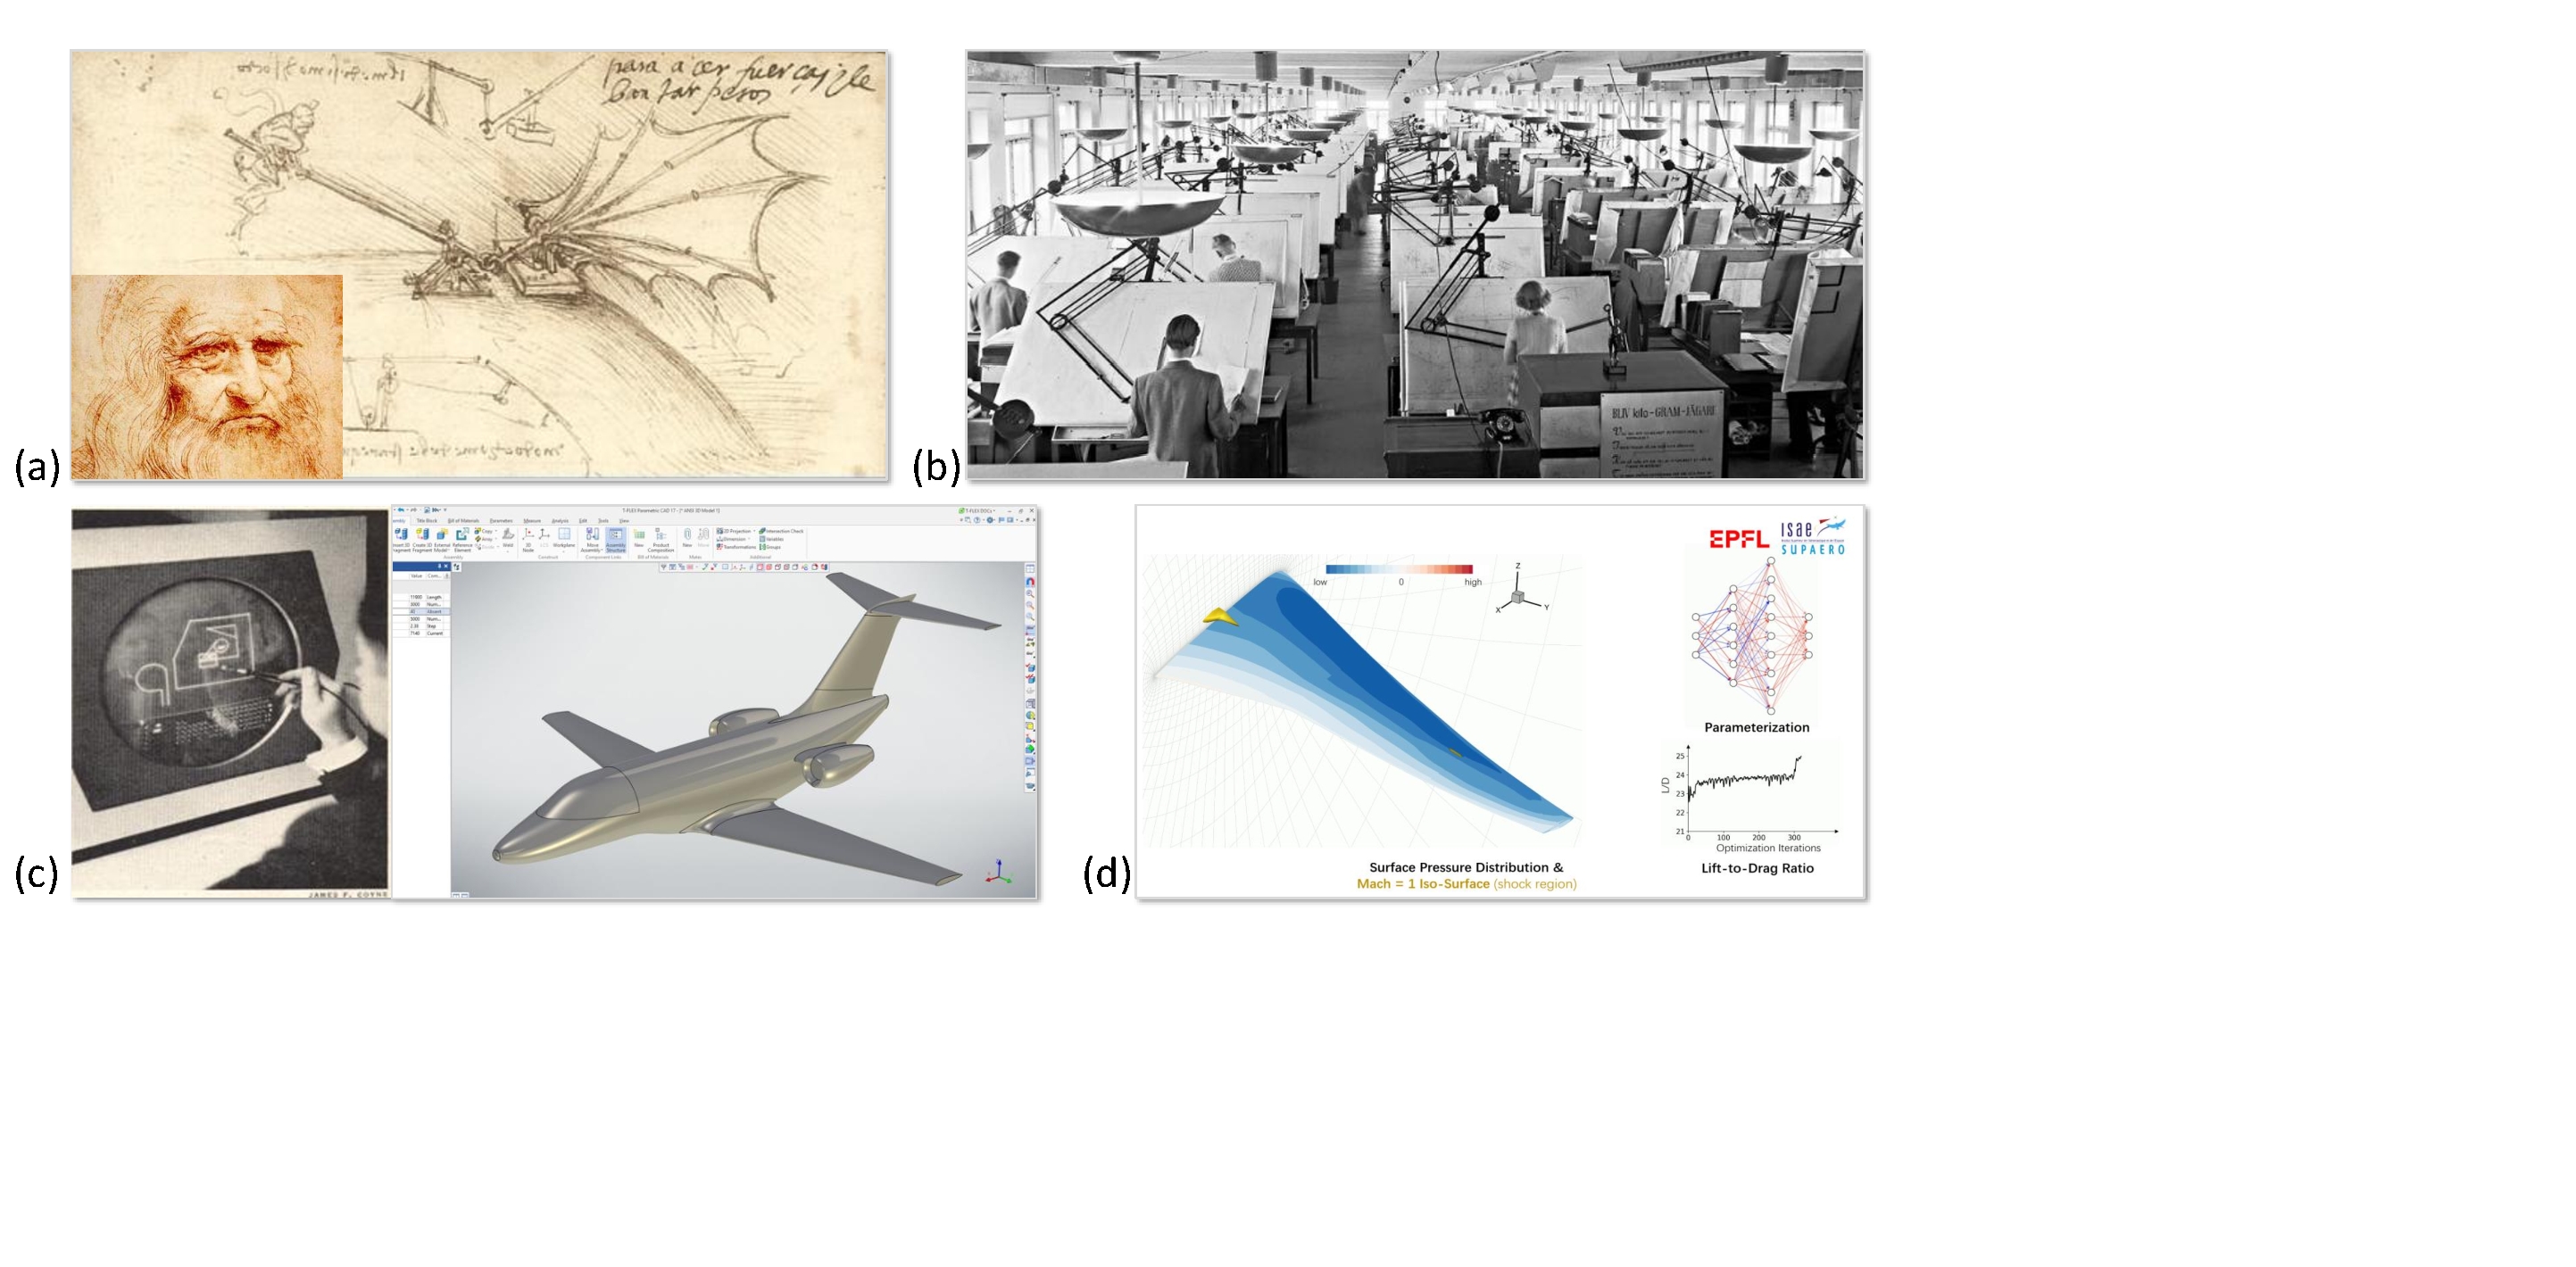
\includegraphics[width=1\linewidth]{chapter2/fig/history.pdf}
    \end{center}
    \vspace{-3mm}
    \caption{
        \small The evolution of engineering design, including (a) design sketches in the Middle Age, (b) modern engineering drawings after the Industrial Revolution, (c) Computer-Aided Design, and (d) AI-driven Computer-Aided Engineering.
    }
    \label{ch2:fig:history}
\end{figure}

The Industrial Revolution catalyzed the emergence of engineering drawing as a formalized practice. To meet the need for precise manufacturing, engineers established strict drafting conventions. The development of descriptive geometry by \textit{Gaspard Monge} in the late 18th century introduced formal methods for projecting 3D objects onto 2D surfaces, providing the mathematical foundation for modern technical drawing.  By the 19th century, technical drawings had adopted unified symbols, dimensioning rules and tolerancing standards to support the complex assemblies. Pioneering engineers like \textit{James Watt} relied on detailed blueprints to manufacture interchangeable parts and complex machinery, such as steam engines. The introduction of drafting tools in the 19th-20th centuries further improved precision. International standards organizations, such as ISO and ANSI, emerged to ensure that engineers around the world interpreted drawings consistently. By the early 20th century, technical drawing had become a highly standardized discipline, transforming engineering design from an art into systematic science.

The advent of digital technology in the mid-20th century further revolutionized engineering design. Early Computer-Aided Design (CAD) systems emerged in the 1960s and 1970s, allowing engineers to create and modify drawings on screen rather than on paper. A milestone was \citet{aa.Sutherland1963}, which demonstrated interactive computer graphics for design. Over the next few decades, CAD technology progressed from 2D drafting in the 1970s to 3D surface and solid modeling systems in the 1980s, and then to feature-based parametric CAD by the 1990s. These tools transformed design practice by allowing faster iterations, easy modifications and three-dimensional visualization. In parallel, advances in computational science led to the rise of Computer-Aided Engineering (CAE) tools for simulation and analysis. By the 1970s, Finite Element Analysis (FEA) and related numerical methods had matured, allowing engineers to predict structural or fluid performance of designs on computers (e.g., contributions by \textit{Antony Jameson} to introducing CFD in commercial aircraft design). Through the 1980s and 1990s, commercial software became mainstream, and CAD and CAE began to integrate. By 2000, the CAD/CAE toolchain was firmly established as an indispensable part of engineering design. This digital transition not only accelerated the design process and reduced human error, but also allowed virtual testing of designs under various conditions before any physical prototype was built.

\section{Modern Developments in Design Representation and Exploration}
\label{ch2:sec:literature_review}

Modern engineering design practice builds upon this long history with advanced techniques for representing designs and exploring the design space. Two aspects are critical in the recent research: (i) how designs and their geometric shapes are represented and parameterized, and (ii) how the design space is explored and optimized to meet performance objectives. Recent progress in AI and computational science has produced a variety of methods in these areas~\cite{aa.Martins2013,aa.Regenwetter2022}. This chapter provides a brief structured review to clarify how each thread of research fits into the broader picture of deep geometric learning for engineering design. The full literatures in each area are presented in the chapter-level reviews that follow.

\subsection{Shape Representation and Parameterization}
A fundamental challenge in engineering design is finding a suitable representation for the geometry of the design. Effective shape parameterization reduces a complex geometric shape to a set of manageable design variables while preserving important features like smoothness and manufacturability. Traditional approaches to shape representation can be divided into explicit (non-data-driven) methods and data-driven methods.
Early explicit parameterization methods originated from computer graphics research. Classic constructive approaches use polynomials or splines, including B-splines~\cite{aa.Braibant1984} and Nonuniform Rational B-Spline (NURBS)~\cite{aa.Farin1995} used in CAD, as well as Parameterized Sections (PARSEC)~\cite{aa.Sobieczky1999} and CST~\cite{aa.Kulfan2008} for 2D airfoils. These methods offer intuitive control and smooth shapes but are often limited to relatively low-dimensional design spaces. Deformative methods provide another option, such as conformal mapping~\cite{aa.Jameson1988}, Hicks-Henne bump function~\cite{aa.Hicks1978} and Free-Form Deformation (FFD)~\cite{aa.Sederberg1986, aa.Kenway2010}. Such non-data-driven parameterizations are widely used in aerodynamic and structural design. However, they require trade-offs between flexibility and complexity: choosing the number of design variables can be crucial, since too few parameters restrict design freedom, while too many parameters make optimization intractable or ill-posed. In addition, these methods lack self-adaptability, as they rely heavily on expert tuning and cannot easily adjust themselves to different types of shapes without manual intervention.

To address the limitations of fixed parameterizations, researchers have turned to data-driven shape representation techniques that leverage existing geometry datasets to find efficient low-dimensional embeddings. Classic machine learning approaches include Proper Orthogonal Decomposition (POD)~\cite{aa.Robinson2001}, Singular Value Decomposition (SVD)~\cite{aa.Poole2015,aa.Li2019,aa.Kedward2020} and Active Subspace Model (ASM)~\cite{aa.Constantine2014,aa.Li2019b,aa.Lukaczyk2014,aa.Namura2017,aa.Grey2018}, while recent deep learning provides richer shape representations through nonlinear latent spaces, including Auto-Encoders~\cite{aa.DAgostino2018,aa.Rios2021,aa.Li2020} and Auto-Decoders (i.e., the Latent Space Model described in Chapter~\ref{ch3}). Such methods can discover a set of latent variables that efficiently describe the data, thereby eliminating the need for explicit shape descriptors. One notable approach is the deep geometric prior/self-prior technique, where a network is trained on a single target shape to encode the geometry, instead of requiring a large dataset. The Direct Mapping Model (Chapter~\ref{ch4}) and DeepGeo (Chapter~\ref{ch5}) are examples of this.

In summary, modern techniques for shape representation span from well-established explicit parameterizations to advanced data-driven and AI-driven models that learn the concept of shapes. Choosing the right representation is important because it directly influences how we explore and optimize within the design space.

\subsection{Design Space Exploration and Optimization}
Design Space Exploration (DSE) is the systematic process of sampling, evaluating and selecting candidate designs to satisfy design objectives. Traditional approaches include Design of Experiments (DoE)~\cite{aa.Fisher1935}, gradient-based optimization and global techniques such as Bayesian optimization~\cite{aa.Kushner1964} or multi-objective evolutionary algorithms (e.g., NSGA-II~\cite{aa.Deb2002}). However, direct optimization on high-dimensional, simulation-based design problems is often computationally prohibitive. Therefore, a significant focus in recent research is on surrogate-assisted design exploration. Surrogate models are approximations of expensive physics-based analyses, which can predict performance rapidly and sometimes provide gradients. Common surrogate modeling techniques include Gaussian processes (Kriging~\cite{aa.Matheron1963}), response surfaces~\cite{aa.Box1951} and neural networks~\cite{ai.Rumelhart1986}. These approaches mitigate the curse of dimensionality to some extent, enabling robust aircraft and automotive optimizations that were once infeasible in reasonable time. The Dfow-SUR model in Chapter~\ref{ch7} builds on this idea by integrating a surrogate model into the loop, demonstrating how surrogate-assisted exploration can accelerate the search for optimal solutions.

Beyond surrogate models, another growing area is the use of deep generative models to directly facilitate DSE. The aim is to create new design candidates that are high-performing and diverse. Typical models include Variational Auto-Encoders (VAEs)~\cite{aa.Yonekura2021,aa.Kou2023,aa.Swannet2024,aa.Wang2022}, Generative Adversarial Networks (GANs)~\cite{aa.Li2020,aa.Li2021,aa.Achour2020,aa.Chen2020} and more recently denoising diffusion models (e.g., DiffAirfoil~\cite{aa.Wei2024}, the work prior to DiffGeo in Chapter~\ref{ch6}). These algorithms can sample the design space broadly, potentially revealing unconventional designs that a deterministic optimizer might not consider. Such generative design models can produce multiple design variants for human or automated screening in early design prototyping and the conceptual design stage. This workflow may transform the traditional paradigm in the near future: instead of iterating on a single design, the generative AI model directly proposes designs expected to meet design objectives, which can then be further verified and fine-tuned through design optimization.

In summary, design space exploration and optimization in the AI era is characterized by hybrid approaches that combine physics-based knowledge with data-driven intelligence. Surrogate models act as efficient physical guidance, while generative models and advanced parameterizations ensure the exploration and exploitation implemented within a feasible and rich design space. These tools together enable us to tackle high-dimensional engineering problems (such as multiple aerodynamic design cases presented in Chapters~\ref{ch5}-\ref{ch7}) that were previously intractable. The future direction is toward automation and intelligence in exploration: rather than manually tuning a design, engineers increasingly rely on algorithms to suggest optimal and innovative designs. This not only accelerates the design cycle but also often yields non-intuitive solutions that human designers might overlook.

The following chapters each contribute to this vision, either by proposing new geometric representations or by introducing novel mechanisms to explore and optimize design geometries. The related work sections in each chapter provide more in-depth discussion.